%%% TODO: ajouter des notions de syntaxe du langage!

\documentclass[English,c,% 't' (resp. 'c') places text vertically at top/center of each slide
% PDF settings
hyperref={%
    pdftitle={FISA-DE2 OOP in Java},%
    pdfauthor={Muller, Gravier, Laforest, Subercaze},%
    pdfsubject={OOP in Java},%
    pdfkeywords={OOP, Java}%
    },%
% To load many pre-defined color names
xcolor={pdftex,svgnames} % dvipsnames, dvipsnames*, svgnames, svgnames*, x11names,
]{beamer}

\usetheme{Copenhagen}
%\setbeamertemplate{footline}[page number]
%\setbeamertemplate{frametitle}[default][center]
% To remove the navigation symbols from the bottom of slides:
\setbeamertemplate{navigation symbols}{}

% Put text more on top of each slide for all slides
\addtobeamertemplate{frametitle}{}{\vspace*{-.7em}}

% Correct French/English indentation and splitting of words
\usepackage{babel}

% Correct management of accentuated chars in input file
\usepackage[utf8]{inputenc}

% Correct font for the generation of docs with accentuated chars
\usepackage[T1]{fontenc}      % Can handle hyphenation of words with accented characters
%%\usepackage[OT1]{fontenc}   % Might generated bad looking PDFs

% Insertion of images generated by external tools
\usepackage{graphicx}
% To generate pretty & scalable images directly in LaTeX
\usepackage{tikz}

% To print numbers correctly
\usepackage{numprint}

\usepackage[absolute,overlay]{textpos}

\usepackage{fourier}

\setbeamercovered{transparent}
\setbeamercovered{invisible}

\AtBeginSection[]
{
   \begin{frame}
       \frametitle{Plan}
       \tableofcontents[currentsection]
   \end{frame}
}

\usepackage{url,manfnt}


% To be able to insert code listing
\usepackage{listings}

\definecolor{dkgreen}{rgb}{0,0.6,0}
\definecolor{gray}{rgb}{0.5,0.5,0.5}
\definecolor{mauve}{rgb}{0.58,0,0.82}

\lstset{frame=none,
  language=Java,
  aboveskip=1mm,
  belowskip=1mm,
  showstringspaces=false,
  columns=flexible,
  basicstyle={\tiny \ttfamily},
  numbers=left,
  numberstyle=\tiny\color{gray},
  keywordstyle=\color{blue},
  commentstyle=\color{dkgreen},
  stringstyle=\color{mauve},
  breaklines=true,
  breakatwhitespace=true,
  tabsize=2
}
\definecolor{algoTitle}{rgb}{0.84,0.83,0.94}

\usepackage{caption}
\DeclareCaptionFont{white}{\color{white}}
\DeclareCaptionFormat{listing}{\colorbox{algoTitle}{\parbox{\textwidth}{\bfseries #1#2 #3}}}
\captionsetup[lstlisting]{format=listing,labelfont=white,textfont=white}

\title[OOP in Java]{Object-Oriented Programming in Java}
\logo{
\includegraphics[width=1cm]{img/logo_tse.png}}
\author{Ch. \textsc{Gravier}, F. \textsc{Laforest}, J. \textsc{Subercaze}, G. \textsc{Muller}}
\institute[TSE/UJM]
{
Télécom Saint-\'{E}tienne\\
Université Jean Monnet\\
\medskip
{\emph{\{pénom.nom\}@univ-st-etienne.fr}}
}
\date[10:07/2019]{7~october~2019}

\begin{document}

%%%%%%%%%%%%%%%%%%%%%%%%%%%%%%%%%%%%%%%%%%%%%%%%%%%%%%%%%%%%%%%%%%%%%%
\begin{frame}
  \maketitle
\end{frame}

%%%%%%%%%%%%%%%%%%%%%%%%%%%%%%%%%%%%%%%%%%%%%%%%%%%%%%%%%%%%%%%%%%%%%%
\begin{frame}{Disclaimer}
This course is an \textbf{introdution}
\begin{itemize}
  \item It does \textbf{NOT} cover \textbf{all} Java
  \item The goal here is to give you enough to understand future TD's intros
  \item A more complete course (French)\\
  {\footnotesize \url{http://jmdoudoux.developpez.com/cours/developpons/java/}}
\end{itemize}
\end{frame}

\section{Introduction}

%%%%%%%%%%%%%%%%%%%%%%%%%%%%%%%%%%%%%%%%%%%%%%%%%%%%%%%%%%%%%%%%%%%%%%
\begin{frame}{Java}
\begin{itemize}
  \item Created in May 1995,
  \vspace{1em}
  \item It's an Object-Oriented language,
  \vspace{1em}
  \item Synthax is close to C,
  \vspace{1em}
  \item It's the most used language in October~2019\\
  \url{https://www.tiobe.com/tiobe-index/}
\end{itemize}
\end{frame}

%%%%%%%%%%%%%%%%%%%%%%%%%%%%%%%%%%%%%%%%%%%%%%%%%%%%%%%%%%%%%%%%%%%%%%
\begin{frame}{Java in~2013}
\begin{itemize}
  \item 97\% of machines have a JVM in enterprises,
  \vspace{1em}
  \item There are more than 9~millions Java developers in the world,
  \vspace{1em}
  \item More than 3 billions mobile devices run Java (Android\ldots{}).
\end{itemize}
\end{frame}

%%%%%%%%%%%%%%%%%%%%%%%%%%%%%%%%%%%%%%%%%%%%%%%%%%%%%%%%%%%%%%%%%%%%%%
\begin{frame}{Characteristics}
\begin{itemize}
  \item Both Compiled (to bytecode) \& Interpreted (on the JVM)
  \vspace{1em}
  \item Portable (independent of the hardware it is executed on)
  \vspace{1em}
  \item Object Oriented, but \textbf{single} inheritance ($\Rightarrow$ \texttt{interfaces})
  \vspace{1em}
  \item Strongly Typed
  \vspace{1em}
  \item Java managed the memory.
\end{itemize}
\end{frame}

%%%%%%%%%%%%%%%%%%%%%%%%%%%%%%%%%%%%%%%%%%%%%%%%%%%%%%%%%%%%%%%%%%%%%%
\begin{frame}{Versions}
There are several distributions of Java
\begin{itemize}
  \item Oracle vs. OpenJDK;
  \item Java Runtime Environment (JRE): only execution environment (JVM);
  $\Rightarrow$ for end users!
  \item Java Development Kit (JDK): set of tools \& APIs to develop in Java;
  $\Rightarrow$ for devs!
  \item Java for enterprises (J2EE): extended JDK with tools \& APIs web development.
\end{itemize}

\textbf{If you install a JDK, do not install a JRE, as it is included in the JDK.}
\end{frame}

%%%%%%%%%%%%%%%%%%%%%%%%%%%%%%%%%%%%%%%%%%%%%%%%%%%%%%%%%%%%%%%%%%%%%%
\begin{frame}{Don't get it wrong}
\begin{center}
JAVA IS NOT JAVASCRIPT\\[1.5em]
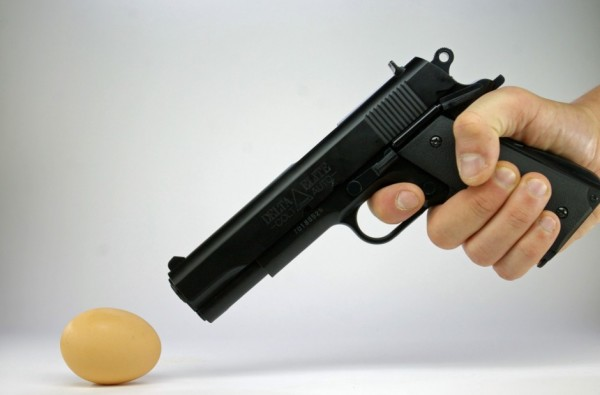
\includegraphics[width=.8\linewidth,height=.6\textheight]{./img/killegg.jpg}
\end{center}
\end{frame}

%%%%%%%%%%%%%%%%%%%%%%%%%%%%%%%%%%%%%%%%%%%%%%%%%%%%%%%%%%%%%%%%%%%%%%
\begin{frame}{Specificities}
The Java platform has some specificities:
\begin{itemize}
  \item It \textbf{compiles} source code into a langage independent of
  the hardware platform it is executed on (bytecode);
  \item This \textbf{bytecode} is executed (\textbf{interpreted}) by a virtual machine (\textbf{JVM} = Java Virtual Machine);
  \item \textbf{Packages} allow to organize code (classes);
  \item \textbf{Classpath} indicates to the compiler \& JVM where to find classes;
  \item \textbf{JAR} (Java ARchive): archive format to
  distribute/deploy executable code as a single file.
\end{itemize}

\end{frame}


\section{Functioning}

\subsection{General Compilation Chain\footnote{Images from "Java Head First'' book.}}

%%%%%%%%%%%%%%%%%%%%%%%%%%%%%%%%%%%%%%%%%%%%%%%%%%%%%%%%%%%%%%%%%%%%%%
\begin{frame}{Compilation Chain -- User's View}

\centering{
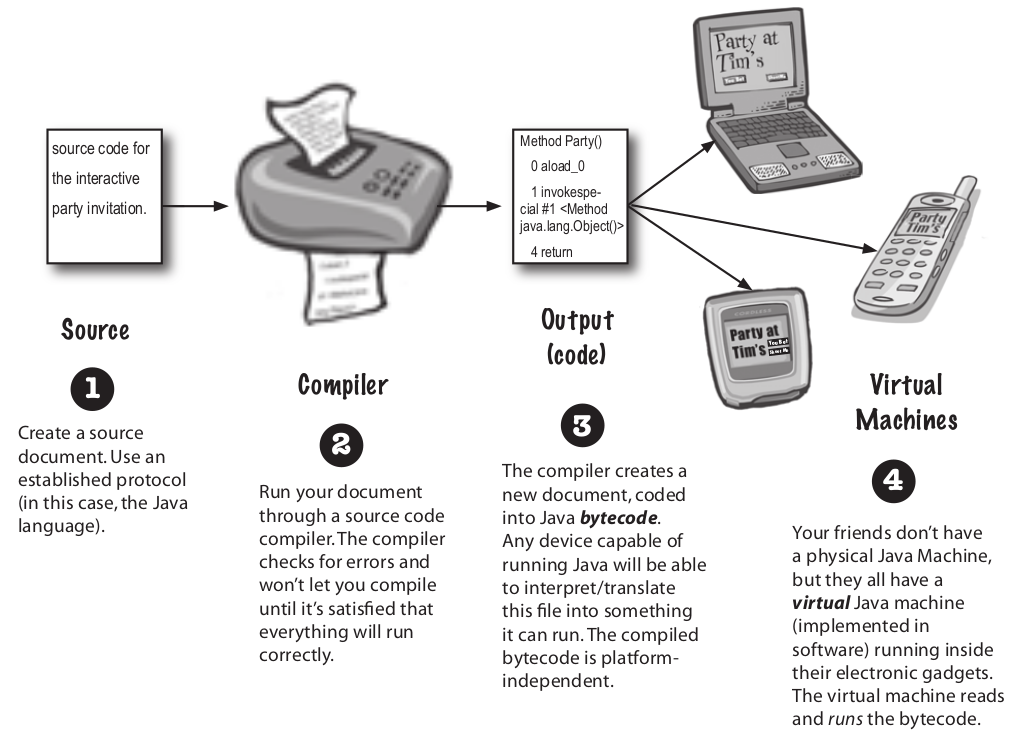
\includegraphics[height=0.85\textheight]{./img/java_intro_compilationchain1.png}
}

\end{frame}
%%%%%%%%%%%%%%%%%%%%%%%%%%%%%%%%%%%%%%%%%%%%%%%%%%%%%%%%%%%%%%%%%%%%%%
\begin{frame}{Compilation Chain -- Developer's View}

\centering{
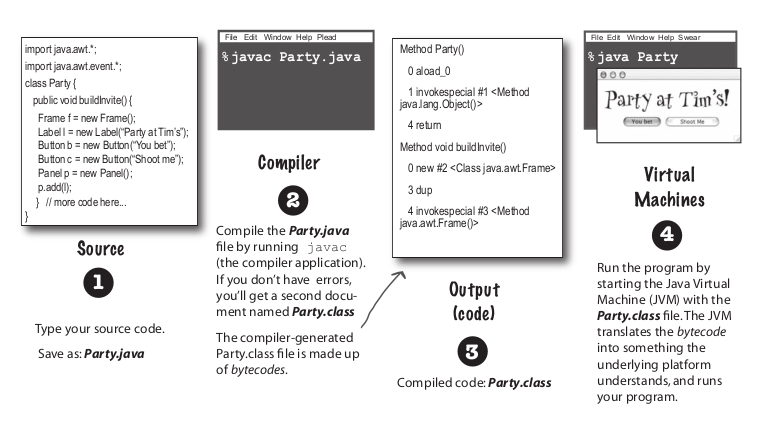
\includegraphics[height=0.85\textheight]{./img/java_intro_compilationchain2.png}
}

\end{frame}
%%%%%%%%%%%%%%%%%%%%%%%%%%%%%%%%%%%%%%%%%%%%%%%%%%%%%%%%%%%%%%%%%%%%%%
\begin{frame}{Source File}

\centering{
  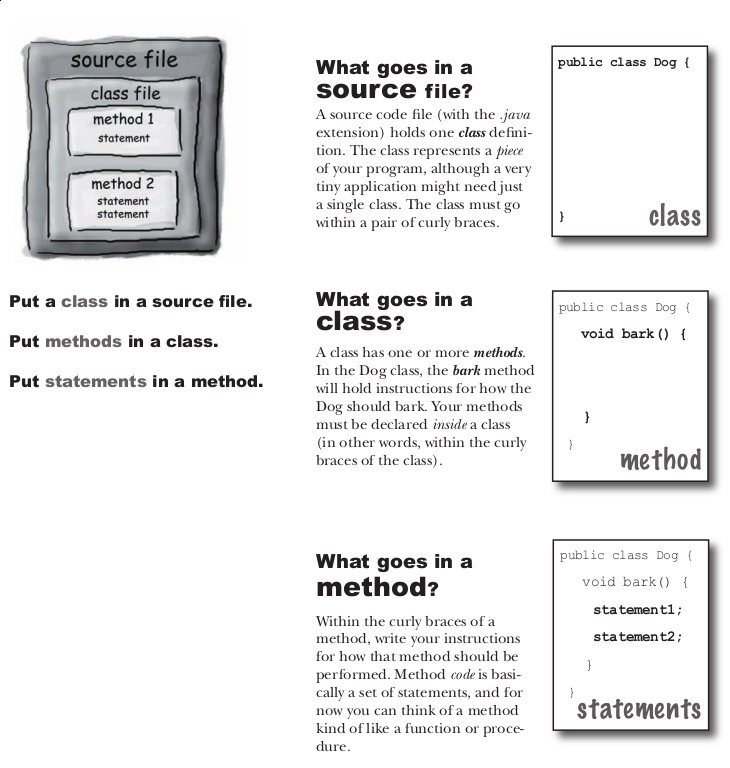
\includegraphics[height=0.8\textheight]{./img/java_intro_sourcefile.png}
}

\end{frame}
%%%%%%%%%%%%%%%%%%%%%%%%%%%%%%%%%%%%%%%%%%%%%%%%%%%%%%%%%%%%%%%%%%%%%%
\begin{frame}{Compilation Chain -- First Run}

\centering{
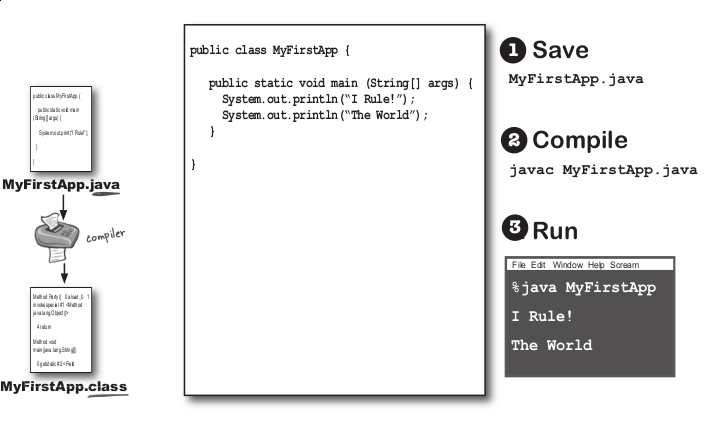
\includegraphics[height=0.85\textheight]{./img/java_intro_compilationchain3.png}
}

\end{frame}
%%%%%%%%%%%%%%%%%%%%%%%%%%%%%%%%%%%%%%%%%%%%%%%%%%%%%%%%%%%%%%%%%%%%%%
\begin{frame}{My First Class}

\centering{
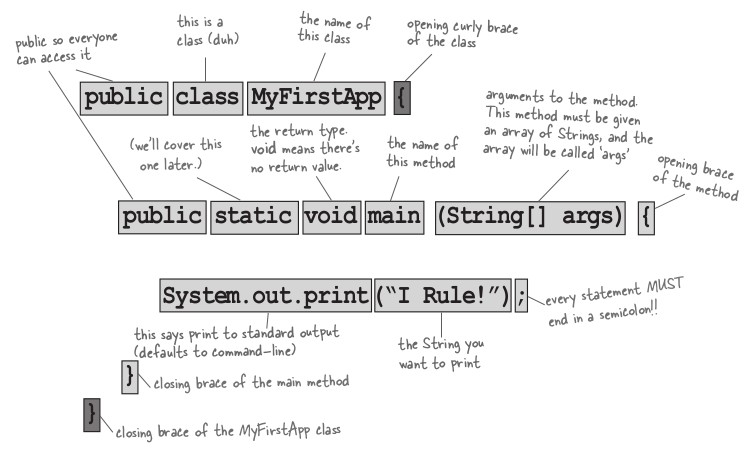
\includegraphics[height=0.85\textheight]{./img/java_intro_class1.png}
}

\end{frame}
%%%%%%%%%%%%%%%%%%%%%%%%%%%%%%%%%%%%%%%%%%%%%%%%%%%%%%%%%%%%%%%%%%%%%%
\begin{frame}{Class File Content}

\centering{
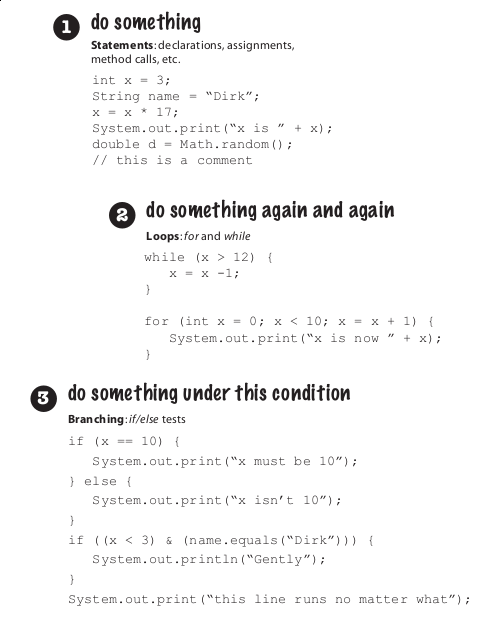
\includegraphics[height=0.8\textheight]{./img/java_intro_class2.png}
}

\end{frame}

\subsection{Keywords}

%%%%%%%%%%%%%%%%%%%%%%%%%%%%%%%%%%%%%%%%%%%%%%%%%%%%%%%%%%%%%%%%%%%%%%
\begin{frame}{Java Keywords}

%\vspace{-.2em}
  { \footnotesize
  \begin{itemize}

    \item (Basic) \textbf{Types}:\\
    \texttt{void}, \texttt{boolean}, \texttt{char}, \texttt{byte},
    \texttt{short}, \texttt{int}, \texttt{float}, \texttt{long},
    \texttt{double}, \texttt{[]}\\
    \texttt{String}, \texttt{List/Set}\ldots{}

    \item \textbf{Packages}: \texttt{import}, \texttt{package}

    \item \textbf{Objects}:\\
    \texttt{interface}/\texttt{class}, \texttt{abstract},
    \texttt{implements}, \texttt{extends}\\
    \texttt{new}, \texttt{this}\\
    \texttt{static}, \texttt{final}

    \item \textbf{Methods}: \texttt{return}, \texttt{super}

    \item \textbf{Visibility}: \texttt{private}, \texttt{public}, \texttt{protected}

    \item \textbf{Control Structures}:\\
    \texttt{for}, \texttt{while}/\texttt{do},
    \texttt{break}/\texttt{continue}\\
    \texttt{if}/\texttt{else}, \texttt{switch}/\texttt{case}

    \item \textbf{Exceptions}:\\
    \texttt{throw}/\texttt{throws}, \texttt{try}/\texttt{catch}/\texttt{finally}

  \end{itemize}
}

\end{frame}

\subsection{Source code, Packages and Bytecode}

%%%%%%%%%%%%%%%%%%%%%%%%%%%%%%%%%%%%%%%%%%%%%%%%%%%%%%%%%%%%%%%%%%%%%%
\begin{frame}{Source code \& bytecode}
\begin{itemize}
    \item Source code is written into files named with extension \texttt{.java};
    \item One (public) class per file;
    \item Each file is named after the public class inside it;
    \item \texttt{javac} (\textbf{java c}ompiler) converts/compiles source code into bytecode;
    \item bytecode files are named with extension \texttt{.class};
    \item This bytecode is executed/interpreted by the JVM.
\end{itemize}
\end{frame}

%%%%%%%%%%%%%%%%%%%%%%%%%%%%%%%%%%%%%%%%%%%%%%%%%%%%%%%%%%%%%%%%%%%%%%
\begin{frame}{On Bytecode and Just-In-Time compilation}

Pros:
\begin{itemize}
    \item Online methods
    \item Eliminate locks
    \item Join adjacent synchronized blocks
    \item Eliminate Dead Code
    \item etc.
\end{itemize}

\pause

Cons:
\begin{itemize}
    \item Increase memory heap,
    \item Loading time,
    \item Even more code modification than traditional compiler.
\end{itemize}

\end{frame}

%%%%%%%%%%%%%%%%%%%%%%%%%%%%%%%%%%%%%%%%%%%%%%%%%%%%%%%%%%%%%%%%%%%%%%
\begin{frame}[fragile]{Exemple}
\begin{lstlisting}[escapechar=\%,label=hellojava,caption=MyClass.java]
public class MyClass {
  public static void main(String[] args) {
    System.out.println("Hello World!");
  }
}
\end{lstlisting}

\bigskip

\begin{itemize}
    \item To compile: \texttt{javac MyClass.java} (creates bytecode into \texttt{hello.class})
    \item To excute: \texttt{java MyClass} (no extension! it the class name!)
\end{itemize}

\end{frame}

%%%%%%%%%%%%%%%%%%%%%%%%%%%%%%%%%%%%%%%%%%%%%%%%%%%%%%%%%%%%%%%%%%%%%%
\begin{frame}{Packages}
\begin{itemize}
    \item Source code is organised in «~packages~»;
    \item This creates a hierarchy of classes that is simpler to apprehend;
    \item This hierarchy is represented as a String, each level is separated by a point (.);
    \item The name of the package corresponds to a sub-directory with the same name;
    \item Example: \\
    \begin{itemize}
      \item \texttt{MyClass} is in the package \texttt{fr.tse.java}
      \item \texttt{MyClass.java} is in the sub-directory \texttt{fr/tse/java/}
  \end{itemize}
\end{itemize}
\end{frame}

%%%%%%%%%%%%%%%%%%%%%%%%%%%%%%%%%%%%%%%%%%%%%%%%%%%%%%%%%%%%%%%%%%%%%%
\begin{frame}[fragile]{Example}
\begin{lstlisting}[escapechar=\%,label=hellopackage,caption=HelloWorld.java.]
package fr.tse.java; // Package declaration implies directory for storage
public class HelloWorld {
  public static void main(String[] args) {
    System.out.println("Hello World");
  }
}
\end{lstlisting}
\end{frame}


%%%%%%%%%%%%%%%%%%%%%%%%%%%%%%%%%%%%%%%%%%%%%%%%%%%%%%%%%%%%%%%%%%%%%%
\begin{frame}{Main packages that already exist in Java}
Some classes are already provided in the Java language API and organized in packages.
\begin{itemize}
  \item java.lang: Basic classes for Java programs (ex: String, Character, Integer\ldots{})
  $\Rightarrow$ imported automatically
  \item java.io: Input/Output (files\ldots{})
  \item java.math: math operations (cos, sin, random\ldots{})
  \item java.util: useful methods, like Collections (lists, sets\ldots{}), logs, etc.
  \item \ldots{}
\end{itemize}
\end{frame}

%%%%%%%%%%%%%%%%%%%%%%%%%%%%%%%%%%%%%%%%%%%%%%%%%%%%%%%%%%%%%%%%%%%%%%
\begin{frame}{How to import classes}
\begin{itemize}
  \item \textbf{Complete list \& description of language packages \& classes}:\\
  \url{http://docs.oracle.com/javase/7/docs/api/}
  \vspace{2em}
  \item It is possible to import external classes (either those provided with Java or one's own) using \texttt{import}
\end{itemize}
\end{frame}


%%%%%%%%%%%%%%%%%%%%%%%%%%%%%%%%%%%%%%%%%%%%%%%%%%%%%%%%%%%%%%%%%%%%%%
\begin{frame}[fragile]{Example of importing Java's class for dynamic arrays (java.util.Vector)}
\begin{lstlisting}[escapechar=\%,label=myvectorpackage,caption=MyVector.java.]
package fr.tse.java;

import java.util.Vector;

public class MyVector {
  public static void main(String[] args) {
    System.out.println("Bonjour");
    Vector<String> v = new Vector<String>();
  }
}
\end{lstlisting}
Description of Java's Vector class:\\
\url{http://docs.oracle.com/javase/7/docs/api/java/util/Vector.html}
\end{frame}

%%%%%%%%%%%%%%%%%%%%%%%%%%%%%%%%%%%%%%%%%%%%%%%%%%%%%%%%%%%%%%%%%%%%%%
\begin{frame}[fragile]{Pointeurs and parameters}

\begin{table}
    \begin{tabular}{|l|l|}
        $C++$           & Java           \\
        \texttt{Pair origin;}     & \texttt{Pair origin = new Pair();} \\
        \texttt{Pair *p, *q, *r;} & \texttt{Pair p, q, r;}            \\
        \texttt{origin.x = 0;}    & \texttt{origin.x = 0;}            \\
        \texttt{p = new Pair;}    & \texttt{p = new Pair();}           \\
        \texttt{p -> y = 5;}      & \texttt{p.y = 5;}                  \\
        \texttt{q = p;}           & \texttt{q = p;}                    \\
        \texttt{r =  \& origin;}  & \texttt{not possible}              \\
    \end{tabular}
\end{table}

\danger{}~If the parameter is a List of Objects, these Objects can be
modified (behind the hood, the List contains references)!!!

\end{frame}


%%%%%%%%%%%%%%%%%%%%%%%%%%%%%%%%%%%%%%%%%%%%%%%%%%%%%%%%%%%%%%%%%%%%%%
\begin{frame}[fragile]{Delete?}
  \vspace{.2em}
\begin{itemize}
    \item The \texttt{new} keyword exists, what about \texttt{delete}?
    \pause
    \item There is no such operator in Java!!!
    \item \textbf{Java manages the memory itself}
    \item With the «~\textbf{Garbage Collector}~» principle
    \item It's a module of the JVM that removes Object from memory when they are not use (referenced) anymore
    \medskip
    \item Pros? Cons?
\end{itemize}
\pause
\centering{
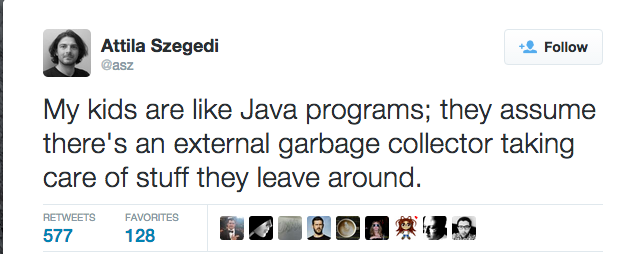
\includegraphics[height=0.4\textheight]{./img/garbage.png}
}
\end{frame}


\subsection{Classpath}


%%%%%%%%%%%%%%%%%%%%%%%%%%%%%%%%%%%%%%%%%%%%%%%%%%%%%%%%%%%%%%%%%%%%%%
\begin{frame}{Archive JAva (JAR files)}
\begin{itemize}
    \item It is possible to assemble all the \texttt{.class} files into an Archive JAva (JAR file, extension \texttt{.jar})\\
    \texttt{jar -cf MyClass.jar ./fr}
    \pause
    \item It is also possible to run/execute this \texttt{jar} file\\
    \texttt{java -jar MyClass.jar}.
    \pause
    \item Under the condition to provide the JVM with the name of the main Class (the one to execute as entry point):
    \begin{itemize}
      \item Create a file \texttt{MANIFEST.MF} in a \texttt{./META-INF/} directory
      \item Append \texttt{Main-Class: fr.tse.java.MyClass} in this file
      \item Add this file to the Java Archive:\\
      \texttt{jar -cmvf  MyClass.jar ./fr}
    \end{itemize}
\end{itemize}
\end{frame}



%%%%%%%%%%%%%%%%%%%%%%%%%%%%%%%%%%%%%%%%%%%%%%%%%%%%%%%%%%%%%%%%%%%%%%
\begin{frame}{Classpath}
\begin{itemize}
    \item OK. Now we have a \texttt{.jar} file that contains multiple \texttt{.class}es.
    \item How to use another project's code that is in another \texttt{jar file}?
    \item It is possible to provide the JVM with a list of external libraries where to look for \texttt{import}ed classes
    \item The list of all the paths for these librairies (Java's and our own's) is called the \textbf{classpath}.
\end{itemize}
\end{frame}


%%%%%%%%%%%%%%%%%%%%%%%%%%%%%%%%%%%%%%%%%%%%%%%%%%%%%%%%%%%%%%%%%%%%%%
\begin{frame}{Classpath}

  The \textbf{classpath} is a list of paths to \texttt{.jar} or
  \texttt{.zip} archives. Each element of the list can be:
\begin{itemize}
    \item A directory: where to look for \texttt{.class} (in their sub-directories)
    \item A \texttt{.jar} or \texttt{.zip} file.
  \end{itemize}

Example of a classpath under Linux or MacOS (le separator is ``:''\footnote{The separator is ``;'' under Windows.}):\\
{\footnotesize \texttt{.:/home/prog/lib/:/usr/lib/java/log4j-1.2.11.jar:../lib-ext/junit.jar}}
\end{frame}

%% HERE

%%%%%%%%%%%%%%%%%%%%%%%%%%%%%%%%%%%%%%%%%%%%%%%%%%%%%%%%%%%%%%%%%%%%%%
\begin{frame}{}
The classpath\\
{\footnotesize \texttt{.:/home/prog/lib/:/usr/lib/java/log4j-1.2.11.jar:../lib-ext/junit.jar}}
is composed of:
\begin{itemize}
    \item \texttt{.class} in current directory  (.)
    \item \textbf{.class} in directory/home/prog/lib/
    \item Classes from archive \texttt{log4j-1.2.11.jar} found in
    \textit{absolute} path \texttt{/usr/lib/java/log4j-1.2.11.jar}
    \item Classes form archive \texttt{junit.jar} find in
    \textit{relative} path \texttt{../lib-ext/junit.jar}
\end{itemize}
\end{frame}


%%%%%%%%%%%%%%%%%%%%%%%%%%%%%%%%%%%%%%%%%%%%%%%%%%%%%%%%%%%%%%%%%%%%%%
\begin{frame}{How to provide the \textbf{classpath} compile/run-time?}
\begin{itemize}
    \item Option \texttt{-classpath} du compilateur
        \begin{itemize}
            \item \texttt{javac -classpath ./:/home/prog/lib/  MyClass.java}
    \end{itemize}
    \item Option \texttt{-cp} of the JVM
    \begin{itemize}
        \item \texttt{java -cp ./:/home/prog/lib/  MyClass}
        \item \texttt{java -cp ./:/home/prog/lib/  fr.tse.java.MyClass}
    \end{itemize}
\end{itemize}

\end{frame}

%%%%%%%%%%%%%%%%%%%%%%%%%%%%%%%%%%%%%%%%%%%%%%%%%%%%%%%%%%%%%%%%%%%%%%
\begin{frame}{Sump Up -- Running Java Manually}
Let's do a live coding demo with Text Editor+Command Line!!!
\begin{itemize}
  \item Open a text editor
  \item Create a \texttt{HelloWorld.java} file + Type a \texttt{HelloWorld} class
  \item Compile with \texttt{javac}
  \item Run with \texttt{java}
  \medskip
  \item Create a \texttt{fr/tse/java} dir hierarchy
  \item Move the class in this directory
  \item Try to run the class $\Rightarrow$ does not work
  \item Add the \texttt{package} directive $\Rightarrow$ it works!!
  \medskip
  \item Create a \texttt{jar} file
  \item Try to execute it with \texttt{java -jar} $\Rightarrow$ does not work
  \item Correct it to add \texttt{./META-INF/MANIFEST.MF} file
\end{itemize}
\end{frame}

%%%%%%%%%%%%%%%%%%%%%%%%%%%%%%%%%%%%%%%%%%%%%%%%%%%%%%%%%%%%%%%%%%%%%%
\begin{frame}{Sump Up -- Eclipse}
Let's do a 2$^{\text{nd}}$ live coding demo, with Eclipse IDE!!!
\begin{itemize}
  \item Start Eclipse
  \item Select workspace (\& accept forever?)
  \item Create a Java/Maven Project
  \item Observe the Project herarchy is automatically created
  \item Create a Package $\Rightarrow$ the dirs are created automatically
  \item Create a Class $\Rightarrow$ file/class names correspond!
  \item Use autocompletion to create \texttt{main}
  \item Use autocompletion to enter \texttt{sysout}
\end{itemize}
\end{frame}

%%%%%%%%%%%%%%%%%%%%%%%%%%%%%%%%%%%%%%%%%%%%%%%%%%%%%%%%%%%%%%%%%%%%%%
\section{Inheritance and Interfaces}

%%%%%%%%%%%%%%%%%%%%%%%%%%%%%%%%%%%%%%%%%%%%%%%%%%%%%%%%%%%%%%%%%%%%%%
\begin{frame}[fragile]{Declare a Class}
\vspace{-1em}
  \begin{lstlisting}[escapechar=\%,label=expers,caption=Person.java,basicstyle=\scriptsize]
public class Person {
    // Attributes
    private String lastName;
    private String firstName;
    // Methods (Constructor)
    public Person (String n, String p) {
        lastName=n;
        firstName=p;
    }
    public void display() {
        System.out.println("First Name: "+firstName+", Last Name: "+lastName);
    }
    public String getName() {
      return name;
    }
}
\end{lstlisting}
\end{frame}


%%%%%%%%%%%%%%%%%%%%%%%%%%%%%%%%%%%%%%%%%%%%%%%%%%%%%%%%%%%%%%%%%%%%%%
\begin{frame}[fragile]{Inheritance -- 1}
\vspace{-1em}
\begin{lstlisting}[escapechar=\%,label=exelv,caption=Student.java,basicstyle=\scriptsize]
public class Student extends Person {
    // Attributes
    private int year;
    // Methods (Constructor)
    public Student(String n, String p, int a) {
       super(n,p);
       year=a;
    }
    @Override
    public void display() {
        System.out.println("Name: "+firstName+" "+lastName+" ("+year+")");
    }
\end{lstlisting}
\end{frame}


%%%%%%%%%%%%%%%%%%%%%%%%%%%%%%%%%%%%%%%%%%%%%%%%%%%%%%%%%%%%%%%%%%%%%%
\begin{frame}{Inheritance -- 2}
\begin{itemize}
  \item Problem:\\
  Parent \& Child classes are \textbf{tightly coupled} $\Rightarrow$ low reusability
  \bigskip
  \item To prevent too much coupling, Java:
  \begin{itemize}
    \item Does \textbf{not} allow multiple inheritance,
    \item Proposes the concept of \texttt{interfaces}.
  \end{itemize}
\end{itemize}
\end{frame}


%%%%%%%%%%%%%%%%%%%%%%%%%%%%%%%%%%%%%%%%%%%%%%%%%%%%%%%%%%%%%%%%%%%%%%
\begin{frame}{Interfaces\footnote{\url{http://imss-www.upmf-grenoble.fr/prevert/Prog/Java/CoursJava/interface.html}}}

 \begin{columns}[t]
  \begin{column}{.55\linewidth}
  \begin{block}{Interfaces in Java}
    An interface defines a behaviour (method prototypes) that must be
    implemented by classes that realize it.
  \end{block}
  \end{column}

  \begin{column}{.40\linewidth}
    \begin{block}{}
      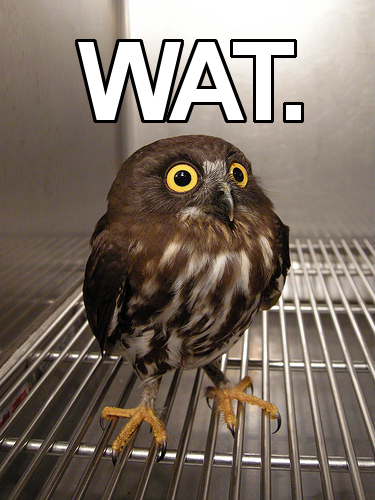
\includegraphics[height=0.6\textheight]{./img/wat.png}
    \end{block}
  \end{column}
 \end{columns}

\end{frame}


%%%%%%%%%%%%%%%%%%%%%%%%%%%%%%%%%%%%%%%%%%%%%%%%%%%%%%%%%%%%%%%%%%%%%%
\begin{frame}{Interfaces}
\begin{itemize}
    \item \textbf{Interfaces} list \textbf{methods} common to all the classes that will implementing it;
    \item Inheritance is reserved for when necessary (ex: a Student \textbf{is a} Person);
    \item Interfaces are \textbf{contracts} that the implementing classes must follow;
    \item Interface do \textbf{NOT} detail the \textbf{implementation} of these methods (i.e. all methods are abstract!)\footnote{This changed in Java~8!};
    \item When a class implements an interface, one can be \textbf{certain} that the methods declared in the interface are present.
\end{itemize}
\end{frame}




%%%%%%%%%%%%%%%%%%%%%%%%%%%%%%%%%%%%%%%%%%%%%%%%%%%%%%%%%%%%%%%%%%%%%%
\begin{frame}[fragile]{Interface: Example -- 1\footnote{\url{http://docs.oracle.com/javase/tutorial/java/concepts/interface.html}}}
\vspace{-1em}
\begin{lstlisting}[escapechar=\%,label=intex,caption=Bicycle.java,basicstyle=\footnotesize]
interface Bicycle {
  // Interfaces do not have attributes

  void changeCadence(int newValue); // Wheel revolutions per minute

  void changeGear(int newValue);

  void speedUp(int increment);

  void applyBrakes(int decrement);
}
\end{lstlisting}

\end{frame}


%%%%%%%%%%%%%%%%%%%%%%%%%%%%%%%%%%%%%%%%%%%%%%%%%%%%%%%%%%%%%%%%%%%%%%
\begin{frame}[fragile]{Interface: Example -- 2}
\vspace{-1.2em}
\begin{lstlisting}[escapechar=\%,label=intex,caption=ACMEBicycle.java,basicstyle=\footnotesize]
class ACMEBicycle implements Bicycle {
    int cadence = 0; // Class has attributes
    int speed = 0;
    int gear = 1;
    void changeCadence(int newValue) { // Methods ARE implemented
         cadence = newValue;
    }
    void changeGear(int newValue) {
         gear = newValue;
    }
    void speedUp(int increment) {
         speed = speed + increment;
    }
    ...
}
\end{lstlisting}
\end{frame}


\section{Documentation -- Javadoc}

%%%%%%%%%%%%%%%%%%%%%%%%%%%%%%%%%%%%%%%%%%%%%%%%%%%%%%%%%%%%%%%%%%%%%%
\begin{frame}{Javadoc tool}
\begin{itemize}
  \item Comments are introduced by:\\
  \texttt{/* \ldots{} */} (multi-line) or \texttt{// \ldots{}} (mono-line)
  \item Class/Attribute/Method \textbf{documentation} is introduced by:\\
  \texttt{/** */}
  \item The documentation can contain HTML tags (\texttt{<b>}, \texttt{<code>}\ldots{})
  \item Documentation comments are split in two parts:
  {\small
    \begin{itemize}
      \item A description in natural language,
      \item A set of tags to identify specific/important information (\texttt{@Author}, \texttt{@Result}\ldots{}).
    \end{itemize}
  }
  \item JDK provides a tool for generating the documentation: \texttt{javadoc} (\textbf{java doc}umentation);
\end{itemize}
\end{frame}



%%%%%%%%%%%%%%%%%%%%%%%%%%%%%%%%%%%%%%%%%%%%%%%%%%%%%%%%%%%%%%%%%%%%%%
\begin{frame}[fragile]{Example\footnote{\url{http://tinyurl.com/2vrongv}}}
\vspace{-1.3em}
{\small
  \begin{lstlisting}[escapechar=\%,label=intex,caption=JavadocExample.java,basicstyle=\footnotesize]
/**
* <p>Returns an Image object that can then be painted on the screen.</p>
* <p>The url argument must specify an absolute {@link URL}.
* The name argument is a specifier that is relative to the url argument.</p>
* @param  url    An absolute URL of the image
* @param  name   The image location relative to the url
* @return        The image at the specified URL
* @see           Image
*/
 public Image getImage(URL url, String name) {
   // do something
   return null;
}
\end{lstlisting}
}
\end{frame}


%%%%%%%%%%%%%%%%%%%%%%%%%%%%%%%%%%%%%%%%%%%%%%%%%%%%%%%%%%%%%%%%%%%%%%
\begin{frame}{Result after calling \texttt{javadoc}: navigable HTML}
\begin{figure}
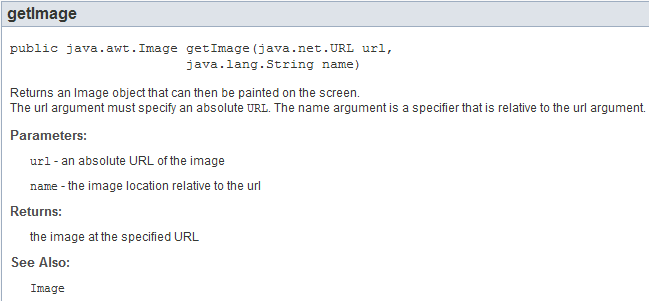
\includegraphics[width=1\textwidth]{./img/javadoc.png}
\end{figure}
\end{frame}


%%%%%%%%%%%%%%%%%%%%%%%%%%%%%%%%%%%%%%%%%%%%%%%%%%%%%%%%%%%%%%%%%%%%%%
\begin{frame}{Possible Tags\footnote{\url{http://tinyurl.com/8uvaclp}}}
\begin{itemize}
    \item \texttt{@author} (classes and interfaces only, required)
    \item \texttt{@version} (classes and interfaces only, required)
    \item \texttt{@param} (methods and constructors only)
    \item \texttt{@return} (methods only)
    \item \texttt{@exception} (@throws is a synonym added in Javadoc 1.2)
    \item \texttt{@see}
    \item \texttt{@since}
    \item \texttt{@serial} (or @serialField or @serialData)
    \item \texttt{@deprecated} (see How and When To Deprecate APIs)
\end{itemize}
\end{frame}


\section{Next steps for the course}

%%%%%%%%%%%%%%%%%%%%%%%%%%%%%%%%%%%%%%%%%%%%%%%%%%%%%%%%%%%%%%%%%%%%%%
\begin{frame}{Remainder}

 \begin{itemize}
  \item 3h CM + 33h TD
  \vspace{3em}
  \item Each TD spans 3h
  \begin{itemize}
    \item Teacher: starts 20 $\rightarrow$ 30 min explanations about a
    specific topic
    \item  Students: 2h30+ of coding practice on the topic
  \end{itemize}
\end{itemize}
\end{frame}


%%%%%%%%%%%%%%%%%%%%%%%%%%%%%%%%%%%%%%%%%%%%%%%%%%%%%%%%%%%%%%%%%%%%%%
\begin{frame}{TDs to come}

{ \small
  \begin{itemize}
  \item TD00: Install and Experiments with Eclipse
  \item TD01: Maven + unit tests
  \item TD02: Files + Exceptions
  \item TD03: POJOs + Wrappers + Strings
  \item TD04: Collections
  \item TD05: Lambdas
  \item TD06: (Data Structures) Graphs
  \item TD07: JDBC
  \item TD08: (GUIs) Swing
  \item TD09: (Algorithms) Convex Hull
  \item TP10: Multithreading
  \item TP11: Introspection
\end{itemize}
}
\end{frame}

\section{Your turn to play with Eclipse!!}

%%%%%%%%%%%%%%%%%%%%%%%%%%%%%%%%%%%%%%%%%%%%%%%%%%%%%%%%%%%%%%%%%%%%%%
\begin{frame}{Goal}
\begin{itemize}
    \item Open Eclipse \& set workspace
    \item Play with Java/Maven Projects
    \item Create Classes, Interfaces\ldots{}
    \smallskip
    \item Create a Hello World project (classes, run configuration\ldots{})
    \smallskip
    \item Create a more complete program: University, Students, Professors\ldots\\
    (with inheritence Professor/Student, interfaces\ldots{})
    \smallskip
    \item Write \& compile Javadoc
    \smallskip
    \item Package the code into a single JAR file \& run it
    \item \ldots
\end{itemize}
\end{frame}


\section*{References}

%%%%%%%%%%%%%%%%%%%%%%%%%%%%%%%%%%%%%%%%%%%%%%%%%%%%%%%%%%%%%%%%%%%%%%
\begin{frame}{References}

%\vspace{-.5em}

{\tiny
\begin{itemize}

  \item \textbf{Eclipse Key Bindings CheatSheet}\\
  \url{https://mootse.telecom-st-etienne.fr/pluginfile.php/9061/mod_resource/content/1/EclipseShortcutCheatSheet.pdf}

  \item \textbf{A few useful CheatSheets}\\
  \url{https://dzone.com/refcardz/getting-started-eclipse}\\
  \url{https://dzone.com/refcardz/core-java}\\
  \url{https://dzone.com/refcardz/getting-started-java-gui}

  \item \textbf{Cool sites}\\
  \url{https://www.baeldung.com/}\\
  \url{https://www.tutorialspoint.com/java/index.htm}\\
  \url{https://jrebel.com/resources/}\\
  \url{https://dzone.com/}\\

  \item \textbf{Complete course}\\
  \url{http://jmdoudoux.developpez.com/cours/developpons/java/}

  \item \textbf{Detailed info on specific topics}\\
  \url{http://mindprod.com/jgloss/jcheat.html}

  \item \textbf{Programming correctly}\\
  \url{https://github.com/GMTSE/ProjetsJavaMaterial/blob/master/JavaByComparisonSumUp.md}

\end{itemize}

}

\end{frame}



%%%%%%%%%%%%%%%%%%%%%%%%%%%%%%%%%%%%%%%%%%%%%%%%%%%%%%%%%%%%%%%%%%%%%%
\begin{frame}
\centerline{The End}
\end{frame}


\end{document}